The decay \btodsphi proceeds via the annihilation of a the constituent quarks in the \Bp meson into
a virtual \Wp boson in the SM.
To acieve the final state, the \Wp decays into a $\cquark\squarkbar$ pair and an additional \ssbar
pair must be \emph{popped} from the QCD field.
This is the only diagram that can perpetuate such a decay because the initial state quarks are all
different to those in the final state.
Annihilation decays of \Bp mesons are rare in the SM due to the magnitude of $|\V{ub}|$ (see
\Eq{eq:th:vub}); in fact, no fully hadronic decays proceeding via annihilation have yet been
observed.

\begin{figure}
  \begin{center}
    %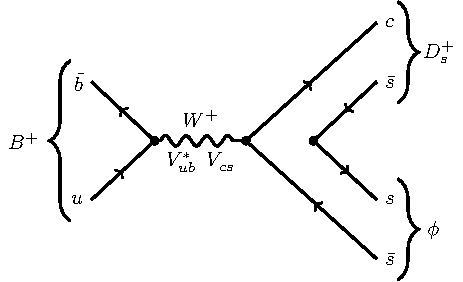
\includegraphics[width=0.48\textwidth]{feynman_dsphi_sm}
    %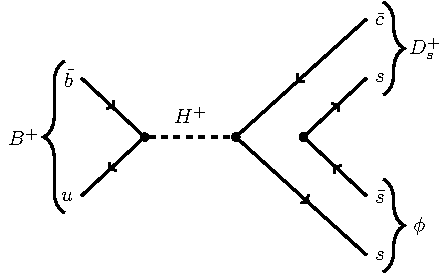
\includegraphics[width=0.48\textwidth]{feynman_dsphi_susy}
    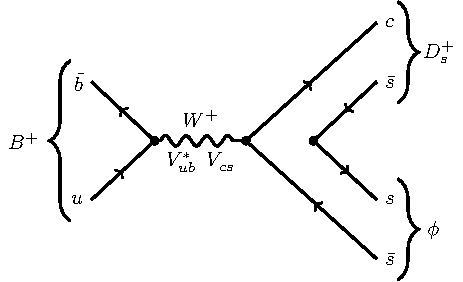
\includegraphics[scale=1]{feynman_dsphi_sm}
    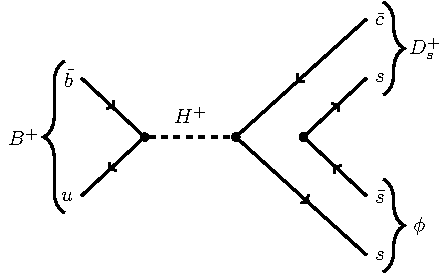
\includegraphics[scale=1]{feynman_dsphi_susy}
    \caption[Feynman diagram for the decay \btodsphi]
    {\small
      A Feynman diagram for the decay \btodsphi being mediated by a
      (left) \Wp in the SM, and
      (right) $H^+$ in SUSY.
    }
    \label{fig:dsphi:feyn}
  \end{center}
\end{figure}

Predictions for the branching fraction $\BF(\btodsphi)$ in the SM are in
the range (1--7)$\e{-7}$~\cite{Zou:2009zza,Mohanta:2002wf,PhysRevD.76.057701,Lu:2001yz}.
However, significant enhancements could be observed were the decay to be mediated by additional BSM
particles; as shown in \Fig{fig:dsphi:feyn}.
One theoretical predicttion would expect that a NP model with two Higgs doublets would have a
branching fraction to be enchaced over the SM by a factor of about ten~\cite{Mohanta:2002wf}:
\begin{align}
  %\BF\big(\btodsphi\big)_\mathrm{SM}&=0.67\e{-6}, \nonumber\\
  %\BF\big(\btodsphi\big)_\mathrm{2HDM}&=\pz8.0\e{-6}, \nonumber\\
  %\BF\big(\btodsphi\big)_\mathrm{RPV}&=3.06\e{-4}.
  \BF\big(\btodsphi\big){\makebox[\widthof{$_\mathrm{2HDM}$}][l]{$_\mathrm{SM}$}}
  &=0.67\e{-6}, \nonumber\\
  \BF\big(\btodsphi\big)_\mathrm{2HDM}
  &=\pz8.0\e{-6}, \nonumber\\
  \BF\big(\btodsphi\big){\makebox[\widthof{$_\mathrm{2HDM}$}][l]{$_\mathrm{SM}$}}
  &=3.06\e{-4}.
\end{align}
%\begin{itemize}
  %\item
%\end{itemize}

The large range in brnaching farction predictions is due to the difficulties in modelling the
hadronizatoin of the final state quarks; the hadronic form-factors lead to large uncertainties.
Calculating the decay dynamics is further complicated because the decay \btodsphi is not fully
factorizable, since the \ssbar pair can come from the final state quarks (factorizable) or the
initial quarks, in which case they contribute to the short range process.

The CP-backward asymmetry, \acp, of the decay is also interesting.
In the SM $\acp=0$, because the Feynamn diagram only contains one phase (in \V{ub}), but
interference from BSM physics diagrams can alter this significatly.
Predicitions from \Ref{Mohanta:2002wf} are:
\begin{align}
  \acp\big(\btodsphi\big)_\mathrm{2HDM}
  &\leq 59\,\%, \nonumber\\
  \acp\big(\btodsphi\big){\makebox[\widthof{$_\mathrm{2HDM}$}][l]{$_\mathrm{RPV}$}}
  &\leq 14\,\%.
\end{align}

There was additional interest in the branching fraction of the decay \btodsphi because of the
historical conflict between the measurements of \V{ub} from incluseive semi-leptonic decays and
from the decay $\decay{\Bp}{\taup\nu_\tau}$, see \Sec{sec:bsm:faisec:bsm:fail}.
The schematic Feynman diagram for \btodsphi is identical to $\decay{\Bp}{\taup\nu_\tau}$, except
that an \ssbar pair must be produced in the case of the former.



%Previous experimental limit by \babar \cite{Aubert:2005gd}
%\begin{equation}
  %\BF\big(\btodsphi\big) < 1.8\e{-6} \qquad \text{90\,\% C.L.}
%\end{equation}






























In theory say that there is no longer a discrepancy (1407.1320).
\cite{PDG2012}
